\documentclass[UTF8]{article}
\usepackage{graphicx}
\usepackage{subfigure}
\usepackage{amsmath}
\usepackage{makecell}
\usepackage[utf8]{inputenc}
\usepackage[space]{ctex} %中文包
\usepackage{listings} %放代码
\usepackage{xcolor} %代码着色宏包
\usepackage{CJK} %显示中文宏包
\usepackage{float}
\usepackage{makecell}
\usepackage{diagbox}
\usepackage{bm}
\usepackage{ulem} 
\usepackage{amssymb}
\usepackage{soul}
\usepackage{color}
\usepackage{geometry}
\usepackage{fancybox} %花里胡哨的盒子
\usepackage{xhfill} %填充包, 可画分割线 https://www.latexstudio.net/archives/8245
\usepackage{multicol} %多栏包
\usepackage{enumerate} %可以方便地自定义枚举标题
\usepackage{multirow} %表格中多行单元格合并
\usepackage{wasysym} %可以使用wasysym里的一堆奇奇怪怪的符号

\geometry{left = 2.5cm, right = 2.5cm, bottom = 2.5cm, top = 3cm}

\definecolor{mygreen}{rgb}{0,0.6,0}
\definecolor{mygray}{rgb}{0.5,0.5,0.5}
\definecolor{mymauve}{rgb}{0.58,0,0.82}

\lstset{
	backgroundcolor=\color{white}, 
	%\tiny < \scriptsize < \footnotesize < \small < \normalsize < \large < \Large < \LARGE < \huge < \Huge
	basicstyle = \scriptsize,       
	breakatwhitespace = false,        
	breaklines = true,                 
	captionpos = b,                    
	commentstyle = \color{mygreen}\bfseries,
	escapeinside=``,
	extendedchars = false,
	frame = shadowbox, 
	framerule=0.5pt,
	keepspaces=true,
	keywordstyle=\color{blue}\bfseries, % keyword style
	language = verilog,                     % the language of code
	otherkeywords={string}, 
	numbers=left, 
	numbersep=5pt,
	numberstyle=\tiny\color{mygray},
	rulecolor=\color{black},         
	showspaces=false,  
	showstringspaces=false, 
	showtabs=false,    
	stepnumber=1,         
	stringstyle=\color{mymauve},        % string literal style
	tabsize=4,          
	title=\lstname,
	texcl=true  
}

%\sum\nolimits_{j=1}^{M}   上下标位于求和符号的水平右端,
%\sum\limits_{j=1}^{M}   上下标位于求和符号的上下处,
%\sum_{j=1}^{M}  对上下标位置没有设定,会随公式所处环境自动调整。

%%%%%%%%%%%%%画图包%%%%%%%%%%%%%
\usepackage{tikz}
%%%%%%%%%%%%%画图背景包%%%%%%%%%%%%%
\usetikzlibrary{backgrounds}

%%%%%%%%%%%%%在tikz中画一个顶点%%%%%%%%%%%%%
%%%%%%%%%%%%%#1:node名称%%%%%%%%%%%%%
%%%%%%%%%%%%%#2:位置%%%%%%%%%%%%%
%%%%%%%%%%%%%#3:标签%%%%%%%%%%%%%
\newcommand{\newVertex}[3]{\node[circle, draw=black, line width=1pt, scale=0.8] (#1) at #2{#3}}
%%%%%%%%%%%%%在tikz中画一条边%%%%%%%%%%%%%
\newcommand{\newEdge}[2]{\draw [black,very thick](#1)--(#2)}
%%%%%%%%%%%%%在tikz中放一个标签%%%%%%%%%%%%%
%%%%%%%%%%%%%#1:名称%%%%%%%%%%%%%
%%%%%%%%%%%%%#2:位置%%%%%%%%%%%%%
%%%%%%%%%%%%%#3:标签内容%%%%%%%%%%%%%
\newcommand{\newLabel}[3]{\node[line width=1pt] (#1) at #2{#3}}

%%%%%%%%%%%%%强制跳过一行%%%%%%%%%%%%%
\newcommand{\jumpLine} {\hspace*{\fill} \par}
%%%%%%%%%%%%%关键点指令,可用itemise替代%%%%%%%%%%%%%
\newcommand{\average}[1]{\left\langle #1\right\rangle }
%%%%%%%%%%%%%表格内嵌套表格%%%%%%%%%%%%%

\newcommand{\keypoint}[2]{$\bullet$\textbf{#1}\quad#2\par}
%%%%%%%%%%%%%<T>平均值表示%%%%%%%%%%%%%
\newcommand{\tabincell}[2]{\begin{tabular}{@{}#1@{}}#2\end{tabular}}%放在导言区
%%%%%%%%%%%%%大黑点item头%%%%%%%%%%%%%
\newcommand{\itemblt}{\item[$\bullet$]}
%%%%%%%%%%%%%大圈item头%%%%%%%%%%%%%
\newcommand{\itemc}{\item[$\circ$]}
%%%%%%%%%%%%%大星星item头%%%%%%%%%%%%%
\newcommand{\itembs}{\item[$\bigstar$]}
%%%%%%%%%%%%%右▷item头%%%%%%%%%%%%%
\newcommand{\itemrhd}{\item[$\rhd$]}
%%%%%%%%%%%%%定义为%%%%%%%%%%%%%
\newcommand{\defas}{=_{df}}
%%%%%%%%%%%%%蕴含%%%%%%%%%%%%%
\newcommand{\imp}{\rightarrow}

%%%%%%%%%%%%%双线分割线%%%%%%%%%%%%%
\newcommand*{\doublerule}{\hrule width \hsize height 1pt \kern 0.5mm \hrule width \hsize height 2pt}
%%%%%%%%%%%%%双线中间可加东西的分割线%%%%%%%%%%%%%
\newcommand\doublerulefill{\leavevmode\leaders\vbox{\hrule width .1pt\kern1pt\hrule}\hfill\kern0pt }
%%%%%%%%%%%%%左大括号%%%%%%%%%%%%%
\newcommand{\leftbig}[1]{\left\{\begin{array}{l}#1\end{array}\right.}
%%%%%%%%%%%%%矩阵%%%%%%%%%%%%%
\newcommand{\mat}[2]{\left[\begin{array}{#1}#2\end{array}\right]}
%%%%%%%%%%%%%可换行圆角文本框%%%%%%%%%%%%%
\newcommand{\ovalboxn}[1]{\ovalbox{\tabincell{l}{#1}}}
%%%%%%%%%%%%%设置section的counter, 使从0开始%%%%%%%%%%%%%
\setcounter{section}{0}

\title{计算机组成原理实验 实验报告}
\date{}

\begin{document}
%%%%%%%%%%%%%科大报告封面%%%%%%%%%%%%%
\maketitle
\begin{figure}[H]
	\centering
	
\includegraphics[width=2.5in]{xiaohui.png}\vspace{0.5cm}\\
	\large{
		实验题目:Lab4 多周期CPU\\
		学生姓名:王章瀚\\
		学生学号:PB18111697\\
		完成日期:\today\\
	}\vspace{2cm}
	
	\large{计算机实验教学中心制\\2019年09月\\}
	\thispagestyle{empty}
	\clearpage  % 清除当页页码
\end{figure}
\newpage

\section{实验题目}
Lab4 多周期CPU

\section{实验目的}
\begin{enumerate}
	\item 理解计算机硬件的基本组成、结构和工作原理;
	\item 掌握数字系统的设计和调试方法;
	\item 熟练掌握数据通路和控制器的设计和描述方法。
\end{enumerate}

\section{实验平台}
Vivado

\section{实验过程}
实验过程主要分为多周期CPU的设计和DBU的设计. 下面分块讲解二者.
\subsection{多周期CPU}
\subsubsection{基本过程}
多周期CPU的部分中, ALU, 寄存器堆, 数据存储器, 指令存储器等结构单元都已经在前面的实验中完成, 这里可以直接调用, 因此不再赘述这几个元件的相关实现.\par
这里需要讲解的部分有: 数据通路, 状态转换, 控制单元及其他代码等.\par
\subsubsection{数据通路}
这里数据通路基本上按照老师的来完成的. 下图是老师给定的数据通路.\par
\begin{figure}[H]
	\centering
	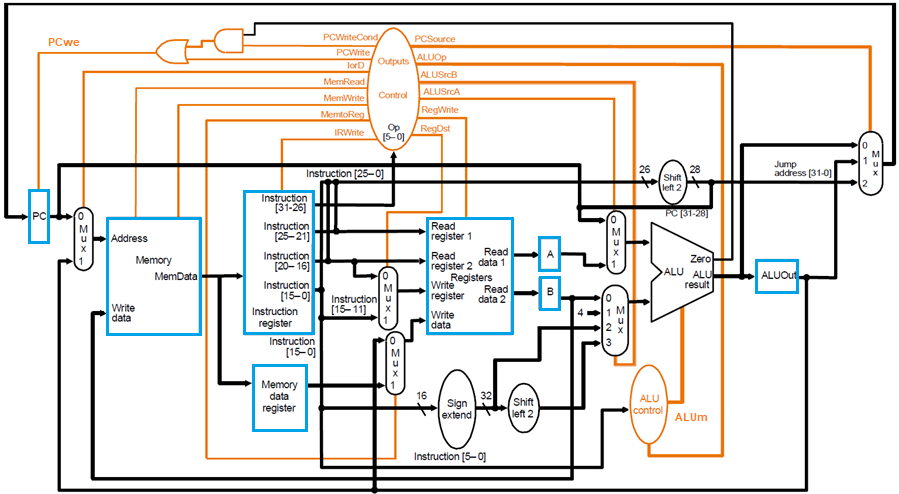
\includegraphics[width=\linewidth]{cpu_data_path_standard.png}
\end{figure}
而我对我完成的代码进行RTL分析, 能够得出下面的数据通路. 其中各个模块的功能已经在图中具体标识了.\par
\begin{figure}[H]
	\centering
	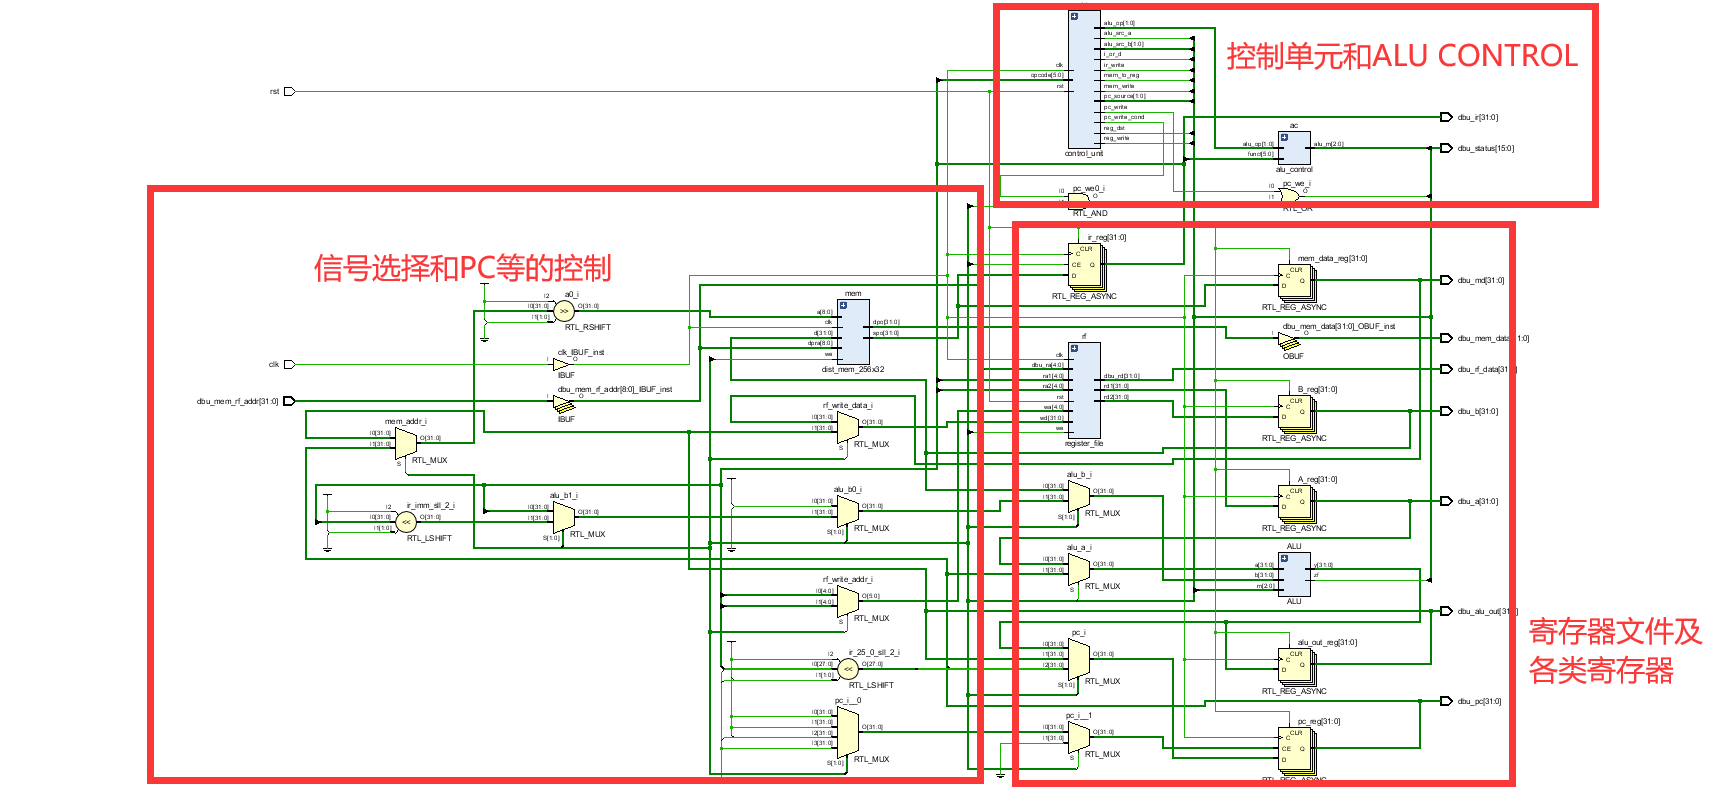
\includegraphics[width=\linewidth]{cpu_data_path.png}
\end{figure}
\subsubsection{状态转换}
多周期的CPU状态机比较复杂, 用graphviz作图, 得到下图.\par
\begin{figure}[H]
	\centering
	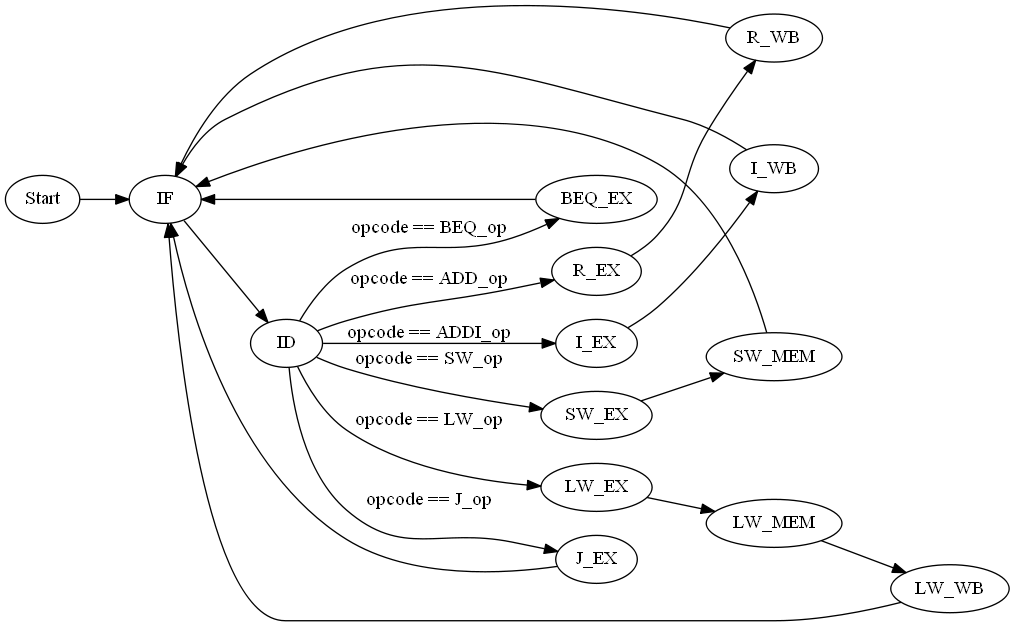
\includegraphics[width=\linewidth]{cpu_phase_diagram.png}
\end{figure}
\subsubsection{代码讲解}
\begin{enumerate}
	\item 数据通路代码\\
	这里只展示CPU内部的数据通路, 传出去给DBU的数据通路就是对应传递即可, 没有什么特别的地方.\\
	而CPU内部数据通路按照老师给出的数据通路进行连接, 其中值得注意的是, 由于存储器的地址应该为字地址, 传入地址的时候需要进行左移两位的操作. 
	并且, 与单周期不同的是, 这里还需要由时钟控制的寄存器的写入.
	代码如下:
	\begin{lstlisting}[language=verilog]
// PC
assign pc_we = pc_write | (pc_write_cond & alu_zero);

// 指令数据存储器
assign mem_addr = i_or_d == 1'b1 ? alu_out : pc;
dist_mem_256x32 mem(.clk(clk), .we(mem_write), 
                    .a(mem_addr >> 2), .d(mem_write_data), .spo(mem_read_data),
                    .dpra(dbu_mem_rf_addr), .dpo(dbu_mem_data));
assign ir_imm = {{16{ir[15]}}, ir[15:0]};
assign ir_imm_sll_2 = ir_imm << 2;

// IR - RF
assign rf_write_addr = reg_dst == 1'b1 ? ir[15: 11] : ir[20: 16];
assign rf_write_data = mem_to_reg == 1'b1 ? mem_data : alu_out;
register_file rf(.clk(clk), .rst(rst), .we(reg_write),
                 .ra1(ir[25: 21]), .rd1(rf_rd1),
                 .ra2(ir[20: 16]), .rd2(rf_rd2),
                 .dbu_ra(dbu_mem_rf_addr), .dbu_rd(dbu_rf_data),
                 .wa(rf_write_addr), .wd(rf_write_data));
assign mem_write_data = B;

// RF - ALU
assign alu_a = alu_src_a == 1'b1 ? A : pc;
assign alu_b = alu_src_b == 2'b00 ? B :
               alu_src_b == 2'b01 ? {{29{1'b0}}, 3'b100} :
               alu_src_b == 2'b10 ? ir_imm : ir_imm_sll_2;
ALU ALU(.m(alu_m), .a(alu_a), .b(alu_b),  
        .y(alu_y), .zf(alu_zero));

// 控制单元
alu_control ac(.alu_op(alu_op), .funct(ir[5: 0]), .alu_m(alu_m));
control_unit cn(.clk(clk), .rst(rst), .opcode(ir[31: 26]),
                .pc_write_cond(pc_write_cond), .pc_write(pc_write),
                .i_or_d(i_or_d), .mem_read(mem_read), .mem_write(mem_write),
                .mem_to_reg(mem_to_reg), .ir_write(ir_write),
                .pc_source(pc_source), .alu_op(alu_op),
                .alu_src_a(alu_src_a), .alu_src_b(alu_src_b),
                .reg_write(reg_write), .reg_dst(reg_dst));

// 一些寄存器的写入
always @(posedge clk) begin
    // Memory Data Register 的写入
    mem_data <= mem_read_data;
    
    // Instruction Register 的写入
    if(ir_write) ir <= mem_read_data;
    else ir <= ir;
    
    // A 和 B 写入
    A <= rf_rd1;
    B <= rf_rd2;
    
    // alu\_out 写入
    alu_out <= alu_y;
end
	\end{lstlisting}
	
	\item PC状态更新\\
	这一部分的代码使得PC状态能够进行状态转移. 和单周期CPU的设计差别不大.
	\begin{lstlisting}[language=verilog]
// PC的更新
assign ir_25_0_sll_2 = ir[25: 0] << 2;
always @(posedge clk, posedge rst) begin
    if(rst) begin
        pc <= 32'h0000_0000;
        mem_data <= 32'h0000_0000;
        ir <= 32'h0000_0000;
        A <= 32'h0000_0000;
        B <= 32'h0000_0000;
        alu_out <= 32'h0000_0000;
    end
    else if(pc_we) begin
        case(pc_source)
            2'b00: pc <= alu_y;
            2'b01: pc <= alu_out;
            2'b10: pc <= {pc[31: 28], ir_25_0_sll_2[27: 0]};
            default: pc <= pc;
        endcase
    end
end
	\end{lstlisting}
	
	\item 控制单元\\
	这部分是CPU的控制单元的代码. 它完成了对整个CPU各个地方的使能等信号的控制.\\
	这里主要就是针对每个指令进行解析, 判断各个状态阶段需要使能哪些信号, 失能哪些信号.\\
	与单周期CPU不同的是, 这里的控制单元需要各种状态的控制, 这里用到的状态如下表.\\
	\jumpLine
	\begin{tabular}{|c|c|}
	\hline
	状态 & 说明 \\
	\hline
	IF & 取指 \\
	\hline
	ID & 解码 \\
	\hline
	R\_EX & R型指令执行 \\
	\hline
	R\_WB & R型指令写回 \\
	\hline
	I\_EX & I型指令执行 \\
	\hline
	I\_WB & I型指令写回 \\
	\hline
	LW\_EX & LW执行 \\
	\hline
	LW\_MEM & LW访存 \\
	\hline
	LW\_WB & LW写回 \\
	\hline
	SW\_EX & LW执行 \\
	\hline
	SW\_MEM & LW访存 \\
	\hline
	BEQ\_EX & BEQ执行 \\
	\hline
	J\_EX & J执行 \\
	\hline
	\end{tabular}\\
	\jumpLine
	为避免一次展示过长代码(且代码将作为附件提交), 这里只分别展示一下各个状态阶段需要输出的控制信号以及状态转换的相关代码.\\
	关于控制信号输出的代码:\\
	\begin{lstlisting}[language=verilog]
// 输出
case(cur_state)
    IF: begin
        mem_read = 1'b1;
        alu_src_a = 1'b0;
        i_or_d = 1'b0;
        ir_write = 1'b1;
        alu_src_b = 2'b01;
        alu_op = 2'b00;
        pc_write = 1'b1;
        pc_source = 2'b00;
    end
    ID: begin
        alu_src_a = 1'b0;
        alu_src_b = 2'b11;
        alu_op = 2'b00;
    end
    R_EX: begin
        alu_src_a = 1'b1;
        alu_src_b = 2'b00;
        alu_op = 2'b10;
    end
    R_WB: begin
        reg_dst = 1'b1;
        reg_write = 1'b1;
        mem_to_reg = 1'b0;
    end
    I_EX, LW_EX, SW_EX: begin
        alu_src_a = 1'b1;
        alu_src_b = 2'b10;
        alu_op = 2'b00;
    end
    I_WB: begin
        reg_dst = 1'b0;
        reg_write = 1'b1;
        mem_to_reg = 1'b0;
    end
    LW_MEM: begin
        mem_read = 1'b1;
        i_or_d = 1'b1;
    end
    LW_WB: begin
        reg_dst = 1'b0;
        reg_write = 1'b1;
        mem_to_reg = 1'b1;
    end
    SW_MEM: begin
        mem_write = 1'b1;
        i_or_d = 1'b1;
    end
    BEQ_EX: begin
        alu_src_a = 1'b1;
        alu_src_b = 2'b00;
        alu_op = 2'b01;
        pc_write_cond = 1'b1;
        pc_source = 2'b01;
    end
    J_EX: begin
        pc_write = 1'b1;
        pc_source = 2'b10;
    end
    default: begin
        {pc_write_cond, pc_write, pc_source,
         i_or_d, mem_read, mem_write, mem_to_reg,
         ir_write, reg_write, reg_dst,
         alu_op, alu_src_a, alu_src_b} = 16'h0000;
    end
endcase
	\end{lstlisting}
	关于状态转移的代码:\\
	\begin{lstlisting}[language=verilog]
// 状态机转移
case(cur_state)
    IF: next_state = ID;
    ID: begin
        case(opcode)
            ADD_op: next_state = R_EX;
            ADDI_op: next_state = I_EX;
            LW_op: next_state = LW_EX;
            SW_op: next_state = SW_EX;
            BEQ_op: next_state = BEQ_EX;
            J_op: next_state = J_EX;
            default: next_state = cur_state;
        endcase
    end
    R_EX: next_state = R_WB;
    R_WB: next_state = IF;
    I_EX: next_state = I_WB;
    I_WB: next_state = IF;
    LW_EX: next_state = LW_MEM;
    LW_MEM: next_state = LW_WB;
    LW_WB: next_state = IF;
    SW_EX: next_state = SW_MEM;
    SW_MEM: next_state = IF;
    BEQ_EX: next_state = IF;
    J_EX: next_state = IF;
    default: next_state = cur_state;
endcase
	\end{lstlisting}
\end{enumerate}
至此, 多周期CPU的代码讲解部分结束.

\subsection{Debug Unit——DBU}
为了便于整个CPU的debug, 需要有一个DBU用以查看各个阶段中的各个输出, 寄存器和存储器的内容等, 以此进行便捷的debug工作.
\subsubsection{基本过程}
这个DBU单元主要有数码管显示控制, LED显示控制, 开关和电键输入解析等构成. 其中维护了一个地址寄存器, 用以查看寄存器文件和数据存储器的存储信息(这个寄存器内容的修改通过上按键和下按键调节).\par
由于没有FPGA开发板, 数码管的显示控制无法进行有效调试, 这里暂不讨论, 但为了证明有做这一项, 还是会把代码贴出.\par
除此之外, 就是一些数据的接线, 以及地址寄存器的内容修改, run信号的生成等. 下面将会讲解.
\subsubsection{数据通路}
DBU这一块的数据通路就由一些CPU模块, 取边沿模块和数码管模块之间的数据通路构成. 为了直观, 下面展示Vivado的RTL分析后的结果.\par
\begin{figure}[H]
	\centering
	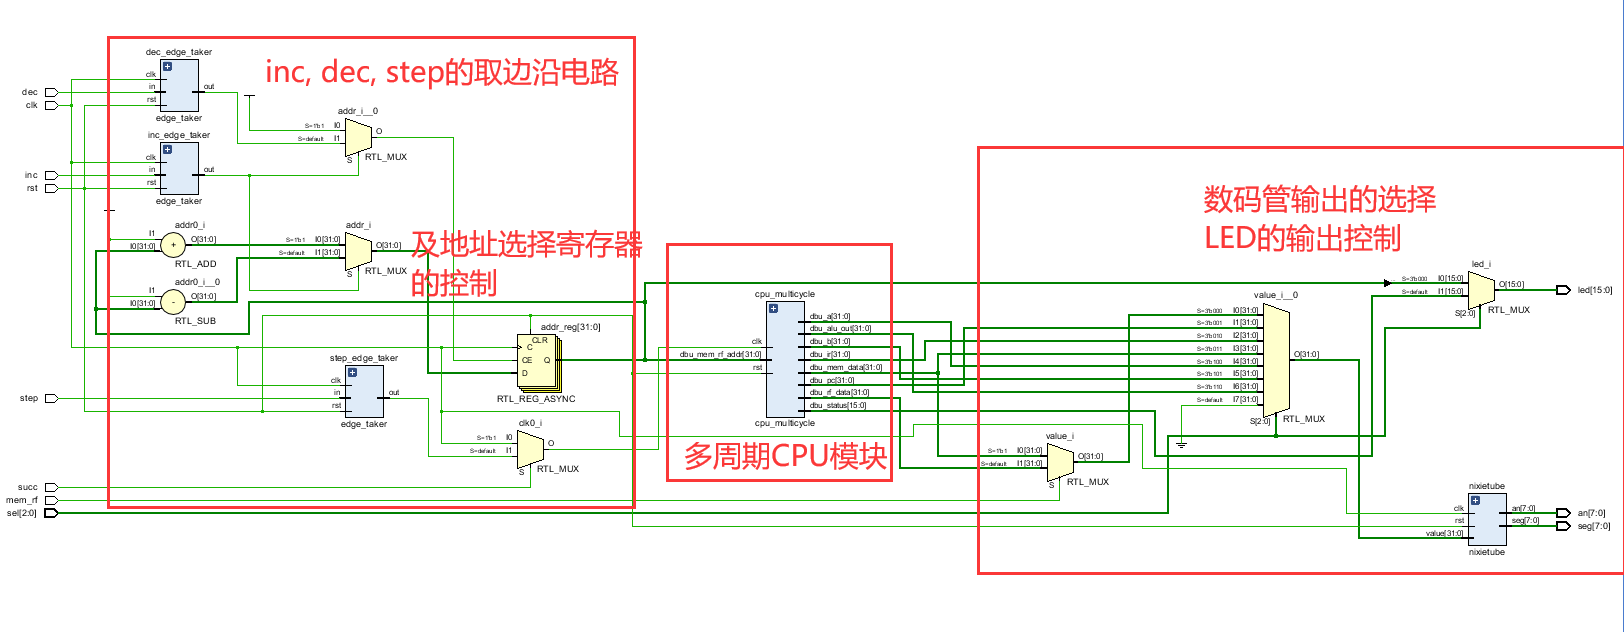
\includegraphics[width=\linewidth]{dbu_data_path.png}
\end{figure}
\subsubsection{状态转换}
DBU这块主要的状态就是选择地址的转换.
\begin{figure}[H]
	\centering
	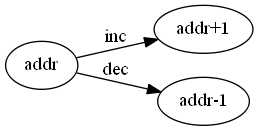
\includegraphics[width=\linewidth/5]{dbu_phase_diagram.png}
\end{figure}
\subsubsection{代码讲解}
\begin{enumerate}
	\item DBU数据通路
	\begin{lstlisting}[language=verilog]
assign dbu_mem_rf_addr = addr;
edge_taker #(.N(1)) inc_edge_taker(.clk(clk), .rst(rst), .in(inc), .out(inc_edge));
edge_taker #(.N(1)) dec_edge_taker(.clk(clk), .rst(rst), .in(dec), .out(dec_edge));
edge_taker #(.N(1)) step_edge_taker(.clk(clk), .rst(rst), .in(step), .out(step_edge));
cpu_multicycle cpu_multicycle(.clk(succ == 1'b1 ? clk : step_edge),
                             .rst(rst),
                             .dbu_mem_rf_addr(dbu_mem_rf_addr),
                             .dbu_rf_data(dbu_rf_data),
                             .dbu_mem_data(dbu_mem_data),
                             .dbu_pc(dbu_pc),
                             .dbu_ir(dbu_ir),
                             .dbu_md(dbu_md),
                             .dbu_a(dbu_a),
                             .dbu_b(dbu_b),
                             .dbu_alu_out(dbu_alu_out),
                             .dbu_status(dbu_status));
// LED显示
assign led = sel == 3'b000 ? dbu_mem_rf_addr : dbu_status;

// 数码管
nixietube nixietube(.clk(clk), .rst(rst), .value(value), .an(an), .seg(seg));
always @(*) begin
    case(sel)
        3'b000: begin
            if(mem_rf) value = dbu_mem_data;
            else value = dbu_rf_data;
        end
        3'b001: value = dbu_pc;
        3'b010: value = dbu_ir;
        3'b011: value = dbu_mem_data;
        3'b100: value = dbu_a;
        3'b101: value = dbu_b;
        3'b110: value = dbu_alu_out;
        default: value = 32'h0000_0000;
    endcase
end
	\end{lstlisting}
	
	\item 地址寄存器的increase和decrease\\
	根据前面数据通路取出的信号边沿, 进行inc和dec操作
	\begin{lstlisting}[language=verilog]
always @(posedge clk, posedge rst) begin
    if(rst) begin
        addr <= 32'h0000_0000;
    end
    else begin
        if(inc_edge) addr <= addr + 1;
        else if(dec_edge) addr <= addr - 1;
    end
end
	\end{lstlisting}
	
	\item 数码管模块的实现\\
	这里直接用了上学期模拟与数字电路实验中完成的数码管, 虽然无从调试, 但应大体正确, 若拿到开发板可进行快速调试与修正.
	\begin{lstlisting}[language=verilog]
module nixietube(
    input clk,
    input rst,
    input [31:0] value,
    output reg [7:0] an,
    output reg [7:0] seg
    );
    
    // 分频计数器
    integer cnt_target_1000HZ;
    integer cnt_1000HZ;
    reg [3:0] digit;
    
    initial begin
        cnt_target_1000HZ = 10000;
        cnt_1000HZ = 0;
        an = 8'h00;
        seg = 8'h00;
    end
    
    always @(posedge clk, posedge rst) begin
        if(rst) begin
            cnt_1000HZ <= cnt_1000HZ + 1;
            an <= 8'b1111_1111;
            seg <= 8'h00;
            digit <= 4'b0000;
        end
        else begin
            if(cnt_1000HZ == cnt_target_1000HZ) begin
                cnt_1000HZ <=  0;
                case(an)
                    8'b1111_1110: begin an <= 8'b1111_1101; digit = value[3:0]; end
                    8'b1111_1101: begin an <= 8'b1111_1011; digit = value[7:3]; end
                    8'b1111_1011: begin an <= 8'b1111_0111; digit = value[11:7]; end
                    8'b1111_0111: begin an <= 8'b1110_1111; digit = value[15:11]; end
                    8'b1110_1111: begin an <= 8'b1101_1111; digit = value[19:15]; end
                    8'b1101_1111: begin an <= 8'b1011_1111; digit = value[23:19]; end
                    8'b1011_1111: begin an <= 8'b0111_1111; digit = value[27:23]; end
                    8'b0111_1111: begin an <= 8'b1111_1110; digit = value[31:27]; end
                    default: begin an <= 8'b1111_1111; digit = 4'b0000; end
                endcase
            end
            else begin
                cnt_1000HZ <= cnt_1000HZ + 1;
            end
        end
    end
    
    always @(*)
    begin
        case(digit)
            4'b0000: seg = 8'b1100_0000;
            4'b0001: seg = 8'b1111_1001;
            4'b0010: seg = 8'b1010_0100;
            4'b0011: seg = 8'b1011_0000;
            4'b0100: seg = 8'b1001_1001;
            4'b0101: seg = 8'b1001_0010;
            4'b0110: seg = 8'b1000_0010;
            4'b0111: seg = 8'b1111_1000;
            4'b1000: seg = 8'b1000_0000;
            4'b1001: seg = 8'b1001_0000;
            4'b1010: seg = 8'b1000_1000;
            4'b1011: seg = 8'b1000_0011;
            4'b1100: seg = 8'b1010_0111;
            4'b1101: seg = 8'b1010_0001;
            4'b1110: seg = 8'b1000_0110;
            4'b1111: seg = 8'b1000_1110;
        endcase
    end
endmodule
	\end{lstlisting}
\end{enumerate}

\section{实验结果}
实验结果部分同样分多周期CPU和DBU两块进行讲解. 但由于DBU完全包含CPU, 故这里不会对多周期CPU部分讲解太多. 若有疑问, 在DBU部分应该会有相应描述.\par
注意, 这里仿真所用的汇编代码为助教提供的代码, 这将极大地方便助教批阅!(见附件)\par
\subsection{多周期CPU}
因为后面的DBU仿真结果会按步骤详细讲解程序运行过程, 所以这一部分就展示一下最后一部分的仿真过程, 并且标识出PC和指令序列(结合汇编程序的beq跳转条件足以证明CPU工作正常), 和最后的程序正确运行时, 存储器的标识.\par
\textbf{注意}, 这里在除了IF阶段, PC对应下来的指令应当是PC+4后的结果, 这是因为PC在IF做了+4, 而非程序有误.\par
仿真结果如下图:\par
\begin{figure}[H]
	\centering
	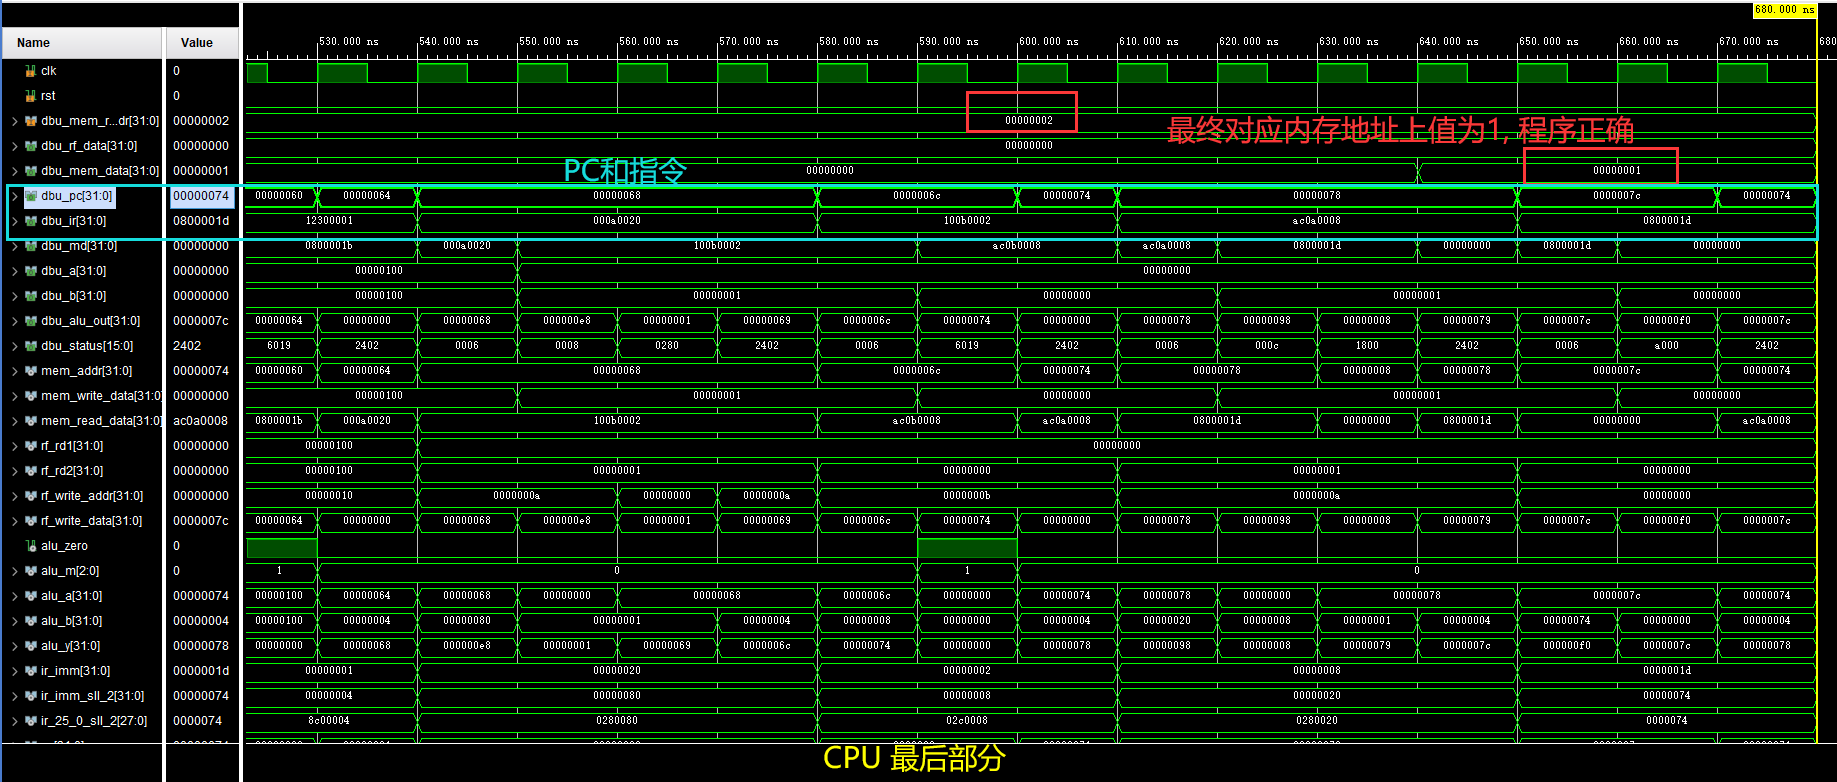
\includegraphics[width=\linewidth]{cpu.png}
\end{figure}
\subsection{Debug Unit——DBU}
这一部分的实验结果比较复杂, 按照助教对汇编代码分的几个部分来描述.
对于DBU\_LED的输出(仿真中变量为dbu\_status), 不再过分陈述, 因为只是进行数据传递, 如果这有错, 那么CPU将无法正常运行.\par
而寄存器文件和数据存储器的内容正确性, 也是程序运行到最后的\_success的必要条件, 因此仿真结果中会有显示, 但并不会做过多说明.\par
下面就用DBU分步讲解整个代码的运行过程!\par
\subsubsection{第一步的jump(到程序开始的地方)}
\begin{figure}[H]
	\centering
	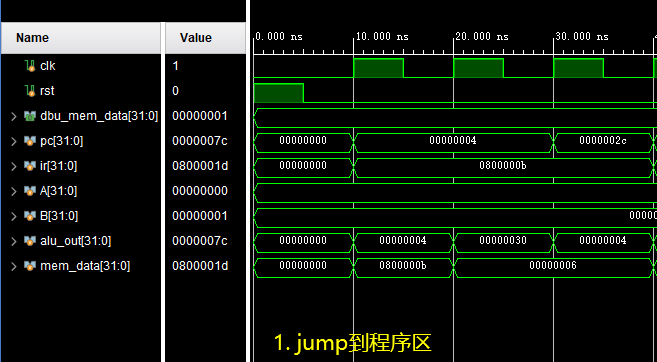
\includegraphics[width=\linewidth]{CPU_1_jump.png}
\end{figure}
\subsubsection{\_start部分}
\_start部分, 对几个寄存器做了addi等操作, 并做了一次lw, 而后beq. 如果能正常beq, 也可以说明代码运行正常.
仿真结果如下. 可以看到alu\_y的结果均正确, 并且pc\_in也表示将会进行程序正确运行时的跳转.
\begin{figure}[H]
	\centering
	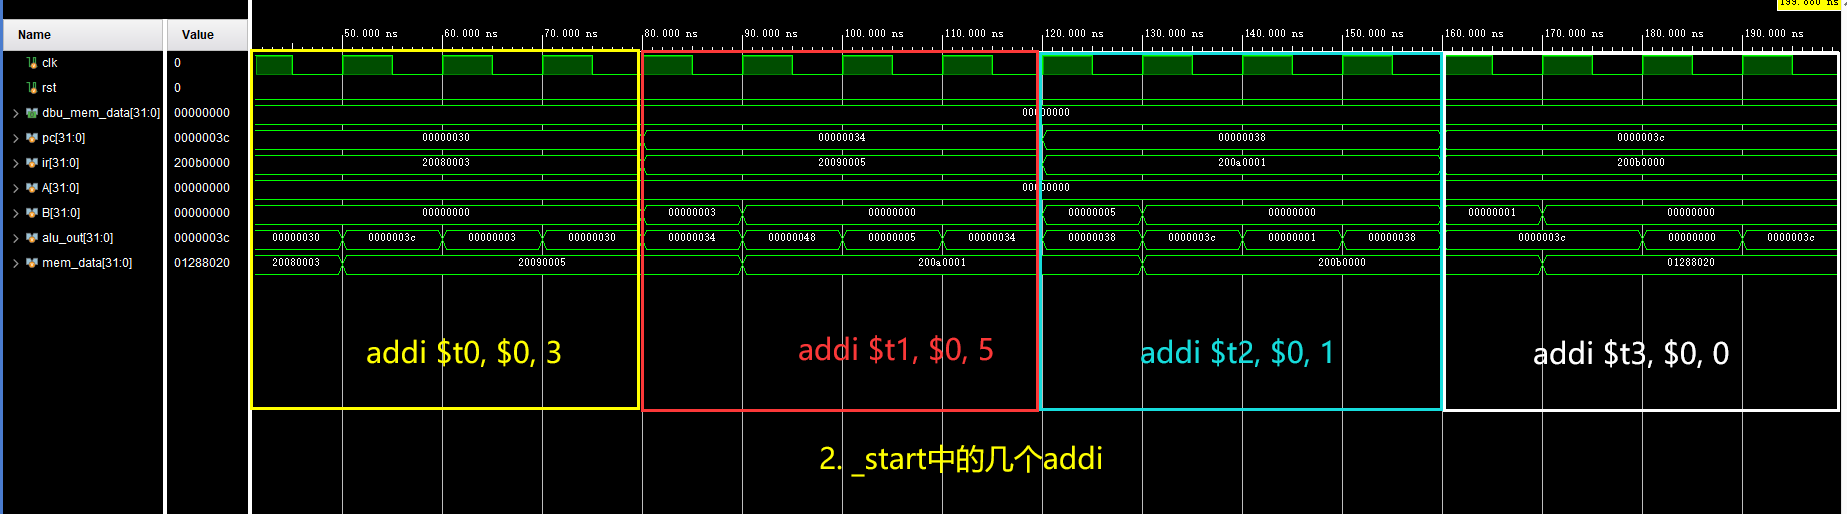
\includegraphics[width=\linewidth]{CPU_3_start_addi.png}
\end{figure}
\begin{figure}[H]
	\centering
	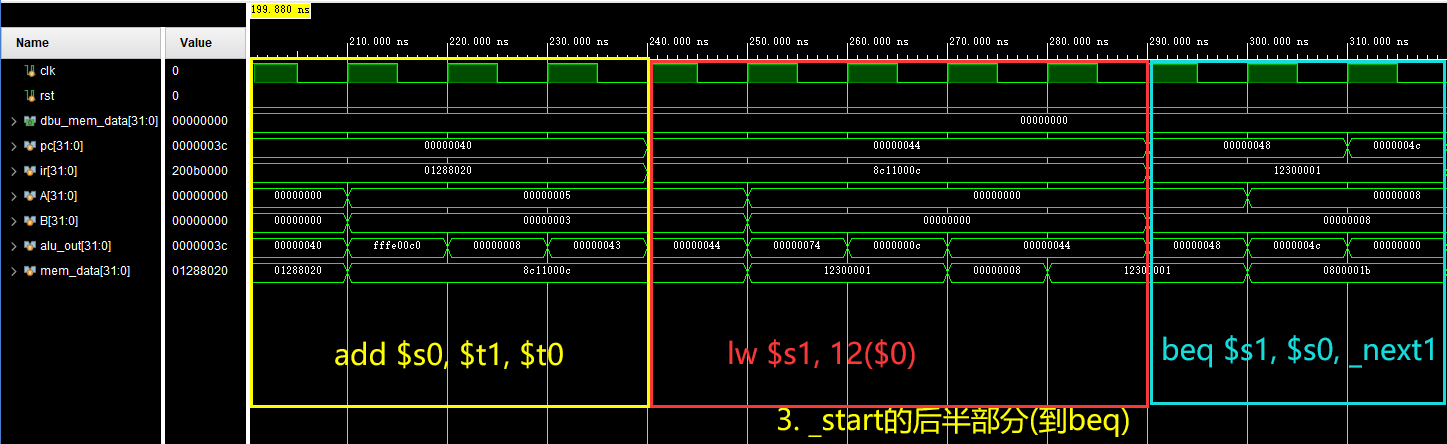
\includegraphics[width=\linewidth]{CPU_4_start_beq.png}
\end{figure}
这一步中, 也展示一下寄存器内容修改的正确性. 同时再次检验inc的可用性.
\begin{figure}[H]
	\centering
	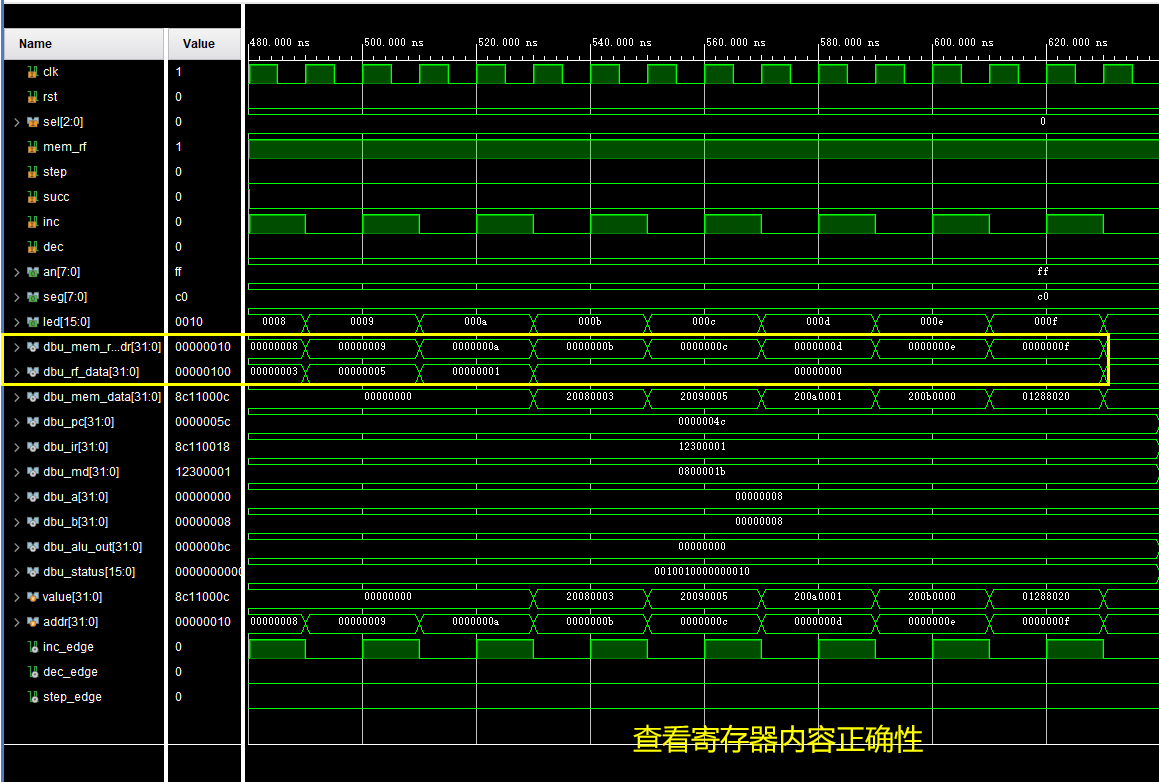
\includegraphics[width=\linewidth]{CPU_2_reg_data.png}
\end{figure}
\subsubsection{\_next1部分}
这一步进行了一些lw操作, 可以检查lw操作的正确处理, 并进行了beq. 同样, 如果能正常beq, 也可以说明代码运行正常.\par
同时, 为了检查step的可行性, 这一部分暂停使用succ, 改用step不断输入, 以逐条执行指令.
\begin{figure}[H]
	\centering
	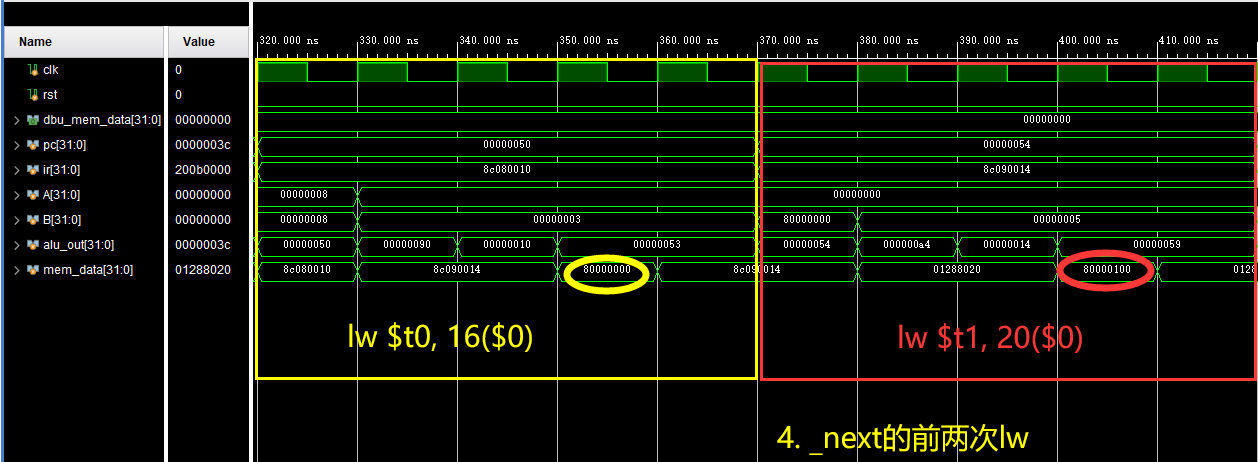
\includegraphics[width=\linewidth]{CPU_5_next1_lw.png}
\end{figure}
\begin{figure}[H]
	\centering
	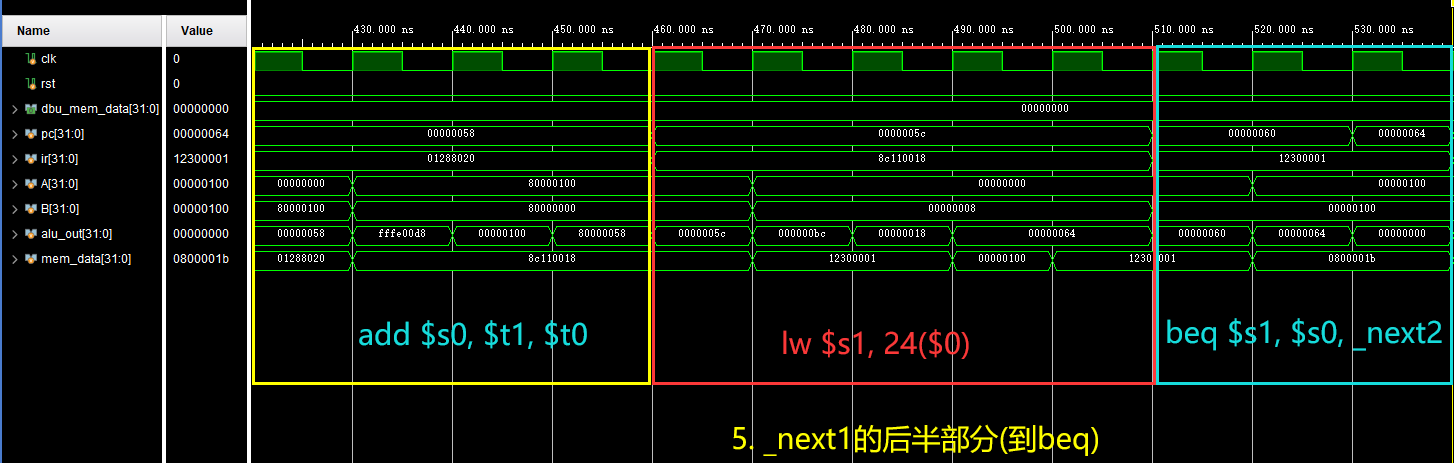
\includegraphics[width=\linewidth]{CPU_6_next1_beq.png}
\end{figure}
\subsubsection{\_next2和\_success部分}
这里主要是检查了寄存器\$0永远为0以及\_success部分的j指令.\par
并且最后展示一下数据存储器地址0x08(字地址为0x2)的数值为1, 表示整个程序运行是正确的.\par
下面展示了寄存器\$0永远为0, 因此能够正确地进行beq. 而在\_success阶段, 数据存储器地址0x08(字地址为0x2)的数值被置为1. 仿真结果如下:
\begin{figure}[H]
	\centering
	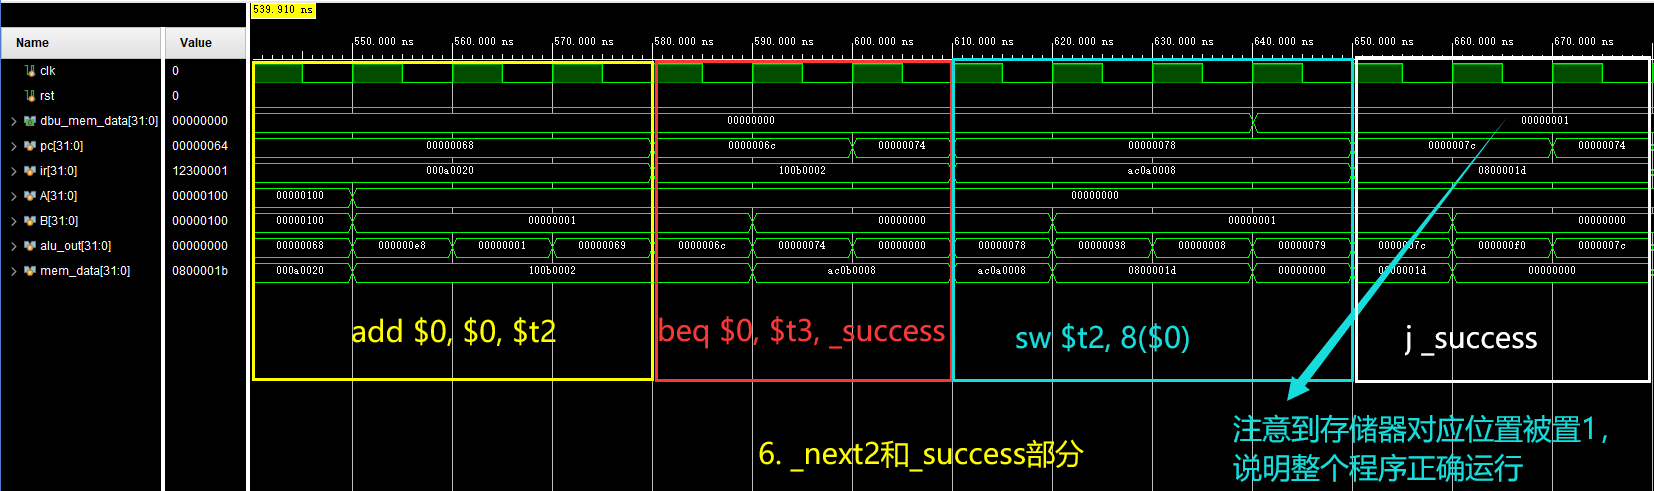
\includegraphics[width=\linewidth]{CPU_7_final.png}
\end{figure}
至此, DBU的仿真过程讲解完毕.

\section{思考题}
\noindent
\textbf{题目}: 修改数据通路和控制器,扩展对其他MIPS指令的支持,并进行功能仿真和下载测试。
实际上, 有了前面对R类, I类, LW, SW, BEQ, J的设计, 要增加一条指令的支持十分简单, 只不过是工程量的问题. 因此为表示我可以完成, 这里加一条\textbf{或指令}. 并将测试代码中\_next2的 "or \$0, \$0, \$t2" 改为 "add \$0, \$0, \$t2".
\begin{figure}[H]
	\centering
	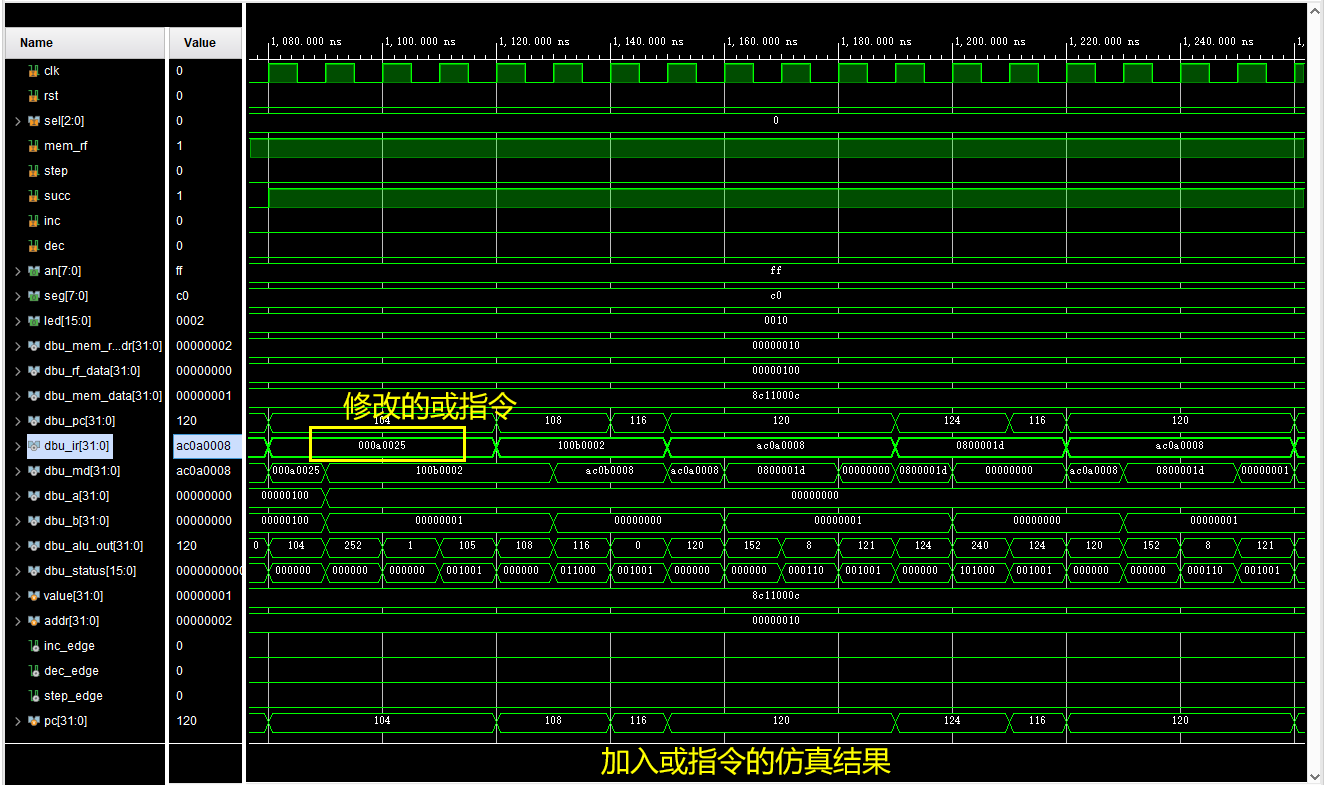
\includegraphics[width=\linewidth]{CPU_OR.png}
\end{figure}
并且从beq的结果也能看出, 这里的执行是正确的.

\section{心得体会}
经过上一次单周期CPU的设计与实现, 已经对CPU的实现有一定理解与基础, 因此这次实现多周期CPU也避免了很多坑.\par
这次实验的收获主要是明白了多周期CPU设计原理, 并且对多周期CPU的了解更进一步. 我想这对后面流水线CPU的设计将有很大帮助.\par
虽然没能拿到FPGA开发板进行测试, 但仿真成功的结果属实令人开心!\par

\section{意见建议}
这次老师和助教们都准备得很充分, 没有什么太多建议.\par

\section{附件}
\begin{figure}[H]
	\centering
	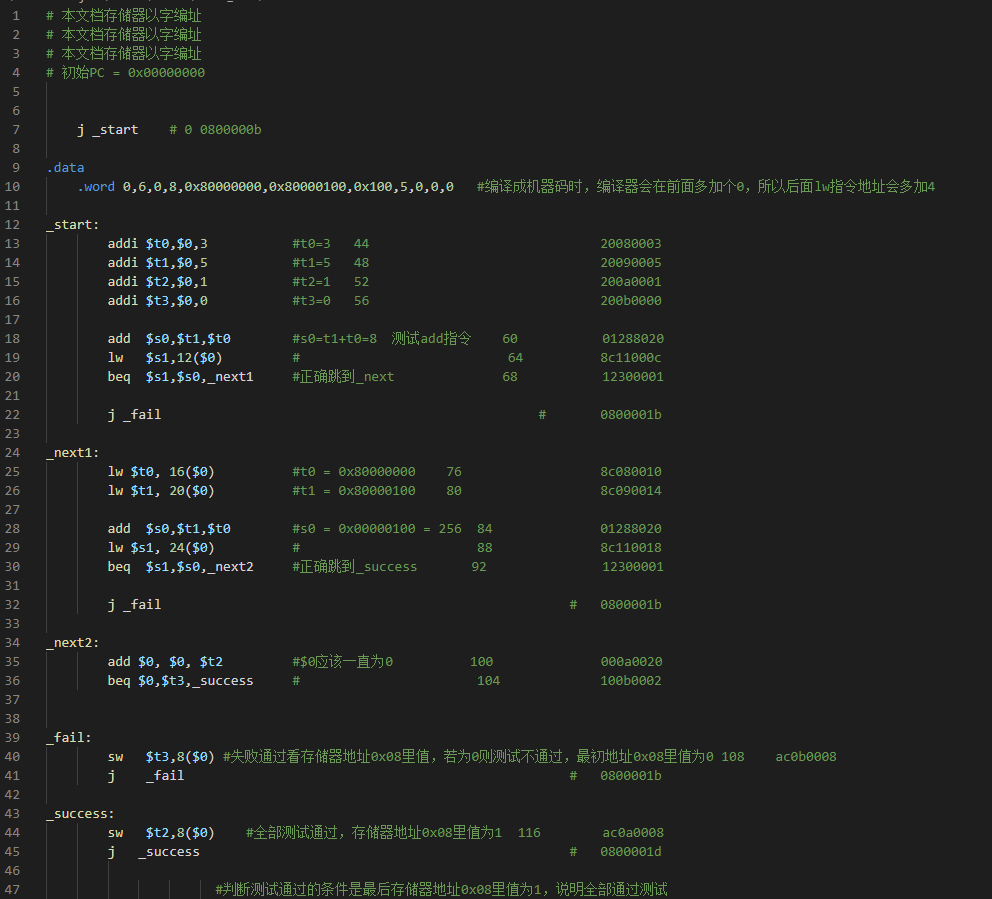
\includegraphics[width=\linewidth]{sim_asm.png}
\end{figure}


\end{document}






